\begin{figure}[ht]
\centering
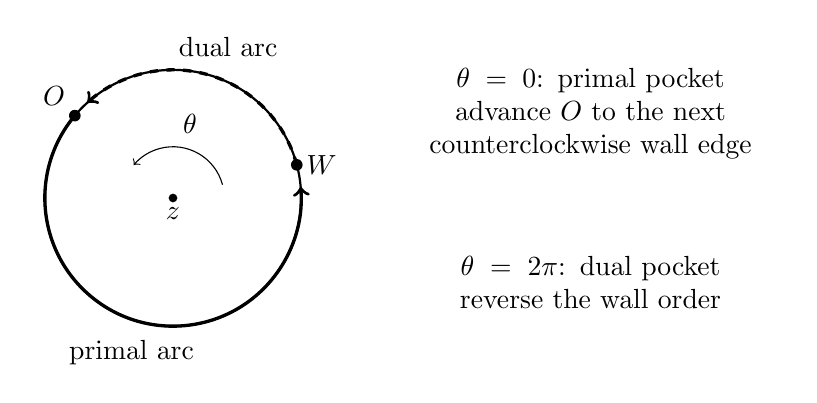
\begin{tikzpicture}[scale=1.05]
 \draw[thick] (0,0) circle (1.55);
 \draw[very thick,dashed,->] (15:1.55) arc (15:132:1.55);
 \draw[very thick,->] (140:1.55) arc (140:365:1.55);
 \fill (0,0) circle (1.5pt) node[below] {$z$};
 \fill (15:1.55) circle (2pt) node[right] {$W$};
 \fill (140:1.55) circle (2pt) node[above left] {$O$};
 \draw[->] (15:.62) arc (15:140:.62);
 \node at (77:.92) {$\theta$};
 \node at (70:1.95) {dual arc};
 \node at (255:1.94) {primal arc};
 \node[align=center,text width=4.8cm] at (5.05,1.02)
 {$\theta=0$: primal pocket\\
  advance $O$ to the next counterclockwise wall edge};
 \node[align=center,text width=4.8cm] at (5.05,-1.02)
 {$\theta=2\pi$: dual pocket\\
  reverse the wall order};
\end{tikzpicture}
\caption{Normalized chart of a two-change component.  The angle
$\theta=O-W$ is measured counterclockwise along the dual arc.
The arrows on the circle indicate boundary order, not strand
orientation.  The forcepoint reset uses the next old-wall edge on the
retained pocket.  A full turn changes the endpoint of the reflected
angular interval.  The drawing is schematic; microscopic tip and
force sides are suppressed.}
\label{tree:figure}
\end{figure}
